\chapter[Pulsar Anatomy]{Pulsar Anatomy}
\label{chapter:PulsarAnatomy}
In this chapter we give
a quick and clear overview of
pulsars as a whole.  Pulsars
are rich with science and each dissected
part of the pulsar has had entire theses
and careers devoted to unraveling its
story.  Admittedly, the following 
sections do not give justice to the plethora
of research done with pulsars.
Further, pulsars are particularly 
interesting because they are objects of extremes.
They probe phases and conditions that
can never be reached in a typical
laboratory.

%\begin{figure}[t!!]
%\begin{center}
%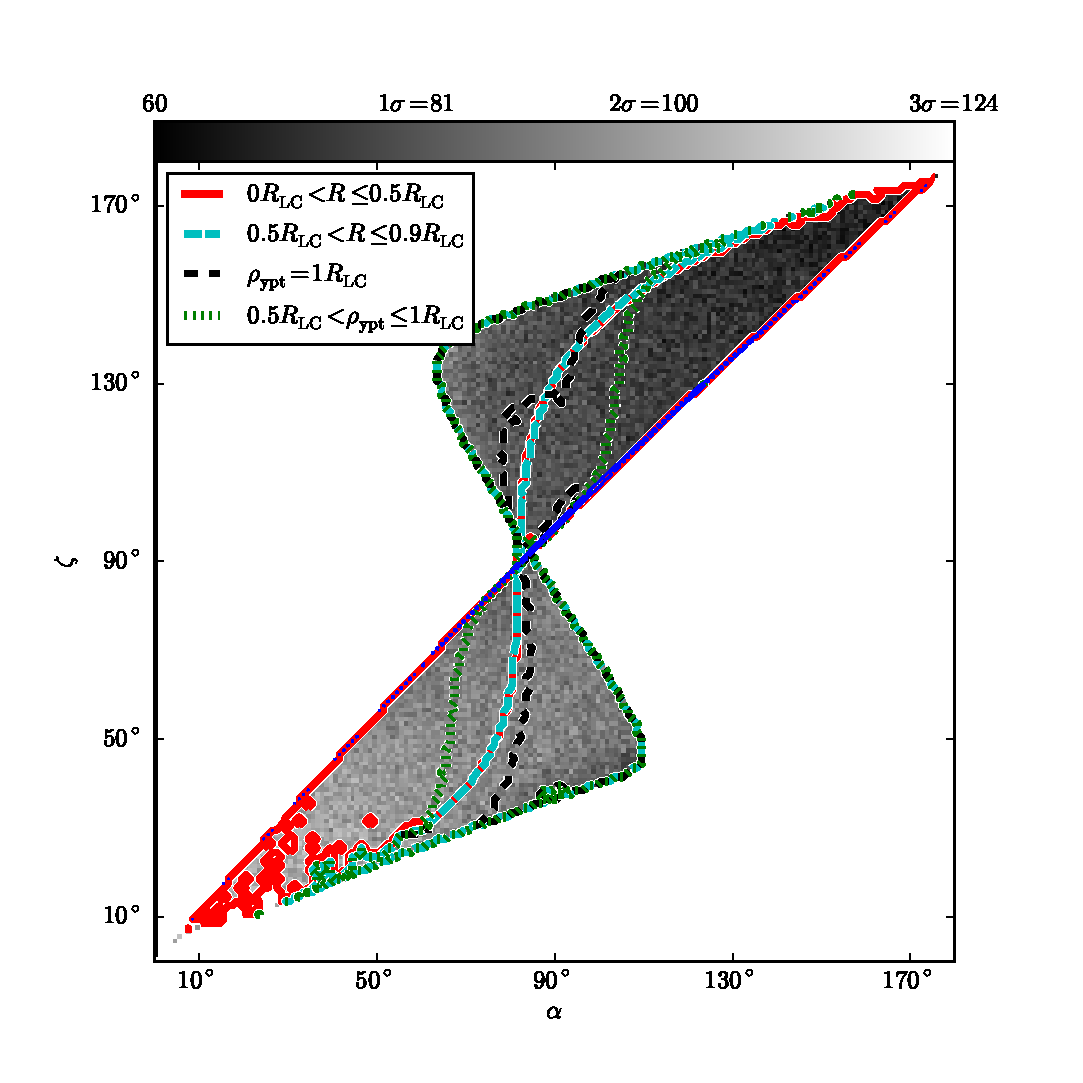
\includegraphics[width=0.98\textwidth]{chapters/pulsarAnatomy/figures/mapB1702allForward.eps}
%\caption{
%\label{}
%}
%\end{center}
%\end{figure}

\begin{figure}[htbp]
\vskip .85\textheight
\special{psfile=chapters/pulsarAnatomy/figures/pulsarAnatomy.eps hoffset=-5 voffset=-10 vscale=65 hscale=65}
\begin{center}
\caption[
Figure of the pulsar anatomy]{Figure of the pulsar anatomy. In Section \ref{sec:originAndSNR} we discuss the supernova remnant and
in Section \ref{sec:PWN} we discuss the pulsar wind nebula.  In Section \ref{sec:pulsarMag}
we explore the basics of the pulsar magnetosphere and review the two acceleration gap locations.
We also briefly summarize the neutron star interior in Section \ref{sec:NSandEOS}.
\label{fig:anatomy}
}
\end{center}
\vskip -0.2truecm
\end{figure}

\section{The Origin of Pulsars and Supernova Remnants}
\label{sec:originAndSNR}
A star will eventually collapse under its own gravity once it has exhausted its energy source.
If the star is massive enough, such a transition will come about violently in a
supernova explosion where most of the mass is expelled in a shell around the position
the star once was. This glowing mass is known as a supernova remnant which
we can continue to observe for 100 to 1000 years after the initial explosion.  The remainder of the
star collapses further either into a black hole or a neutron star depending on the
original mass of the star.  Since most of the angular momentum is conserved, the
much smaller, denser neutron star has a very small rotational period.
Additionally, magnetic flux is also conserved resulting in large magnetic fields.

For a normal star, the radius $R_0$ is $10^5$ to $10^8$ km and
the rotational period $P_0$ is a month to several years.
Equations for conservation of angular momentum and magnetic flux are
\begin{equation}
M R^2_0 \Omega_0=M R^2 \Omega
\end{equation}
\begin{center}
and
\end{center}
\begin{equation}
R^2_0 B_0 = R^2 B.
\end{equation}
With some physical considerations
(e.g. a very small period would result
in the star falling apart) it follows that
\begin{equation}
P \sim (R/R_0)^2 P_0 \sim .001 - 1 \quad \rm{seconds}\\\\
\end{equation}
\begin{center}
and
\end{center}
\begin{equation}
B \sim (R_0/R)^2 B_0 \sim 10^{10}-10^{12} \quad \rm{Gauss}.
\end{equation}

The rotational period of pulsars range from a couple of milliseconds to
several seconds.  For instance, PSR J$1748-2446$ad has one of the shortest
 periods known at $1.395$ ms \citep{hessels2006radio}.
The magnetic fields of pulsars are around $10^{10}$ to $10^{12}$ Gauss.
Magnetars, neutron stars with extremely strong magnetic fields, are said to have
magnetic fields of up to $10^{15}$ Gauss.  (The magnetic field of the Earth is
around $\sim 0.4$ Gauss and the magnetic field of the sun is around $\sim 1$ Gauss, for reference.)

One of the most massive pulsars is PSR J$1311-3430$ which has a mass
of $2.15$ to $2.7M_{\odot}$ (solar mass) from spectroscopic measurements \citep{romani2012psr}.
But the radius of neutron stars are tiny compared to solar radius at around $1.4\times10^{-5} R_{\odot}=10$km.
(The circumference is approximately the distance from
San Fransisco to San Jose.)

Neutron stars were first predicted as a result of
supernovae by \cite{baade1934super} many years before they
were observed.
Although the first supernovae was observed thousands of years ago,
the first pulsations (in radio) from pulsars were not observed 
(or more accurately, \textit{recognized}) until
relatively recently in 1967 to 1968.
The first correct and complete explanation of pulsars and their
connection to neutron stars followed rapidly by Gold and Pacini
\citep{pacini1967energy, gold1968rotating, pacini1968rotating}.
Today, the number of radio detected pulsars is in the low thousands and the number of energetic $\gamma$-ray
detected pulsars is in the low hundreds.
The number of galactic neutron stars is estimated at $\sim10^9$ although
how many are actually visible from Earth depends on a number of caveats \citep{colpi1998elusiveness}.




\section{Pulsar Wind Nebula}
\label{sec:PWN}

Unlike supernova remnants,
the pulsar wind nebulae are continuously renewed in energy
and are visible for much longer than supernova remnants.

Energy from the pulsar rotation is dissipated into the pulsar wind.
This dissipated spin down energy is given as
\begin{equation}
\dot{E}=I \Omega \dot{\Omega}
\end{equation}
where $I$ is the moment of inertia of the spinning neutron star and $\Omega$
is the angular frequency of the rotation.

The angular frequency and change in the angular frequency are
assumed to be related to each other as
\begin{equation}\label{eq:angFreq}\dot{\Omega} \propto \Omega^n\end{equation}
where $n$ is the braking index.
Using this relationship, one can solve for the age of the pulsar.

\begin{figure}[t!!]
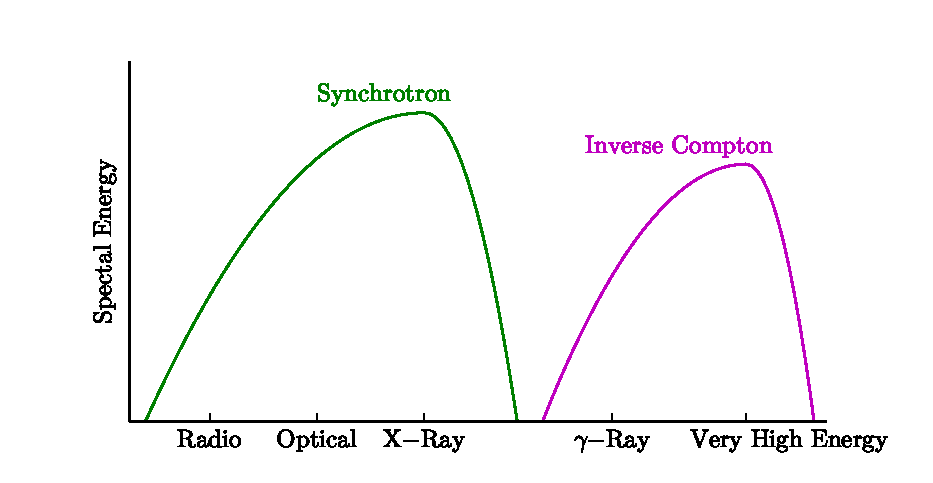
\includegraphics[width=.95\textwidth]{chapters/pulsarAnatomy/figures/spec.eps}
\caption[Typical pulsar wind nebula energy spectrum]{
\label{spec} Typical pulsar wind nebula energy spectrum.
Inspired by Figure 1.1 of \cite{vanEttenPhd2012}.}
\end{figure}

Interaction of this outflow with surrounding medium creates emission.
Particles interact with magnetic fields and photons to produce
synchrotron (very relativistic and ultra-relativistic electrons
gyrating in a magnetic field)
and inverse Compton (scattering of low energy photons
to high energy by ultra-relativistic electrons) emission. For
younger pulsars, this medium includes the cold supernova ejecta
beyond the termination shock.
Termination shock forms where the ram pressure of the wind 
balances the pressure of the surrounding medium.  
Figure~\ref{spec} shows a typical energy spectrum of a pulsar
wind nebula.


Of particular interests to polarization and geometric modeling
(the main theme of this thesis)
is the X-ray torus of pulsar wind nebulas which is further discussed
in Section \ref{subsec:ToriModeling}.
For more detailed overview of pulsar wind nebula see \cite{vanEttenPhd2012}
and
\cite{gaensler2006evolution}.

\section{Pulsar Magnetosphere}
\label{sec:pulsarMag}
The simplest model of the pulsar magnetosphere is
a very large magnetic (static) dipole in space.  Many of 
the well-used analytic formulations for analysis of pulsar
data are based on this simplistic assumption. 
We will discuss some of the models in later chapters.

The magnetic field of a \textit{rotating} vacuum dipole are given as

\begin{equation}
\label{eq:magField}
\vec{B}=-\frac{ \vec{m}(t_{\rm r}) +r\dot{\vec{m}}(t_{\rm r}) + r^2\ddot{\vec{m}}(t_{\rm r})}{r^3} + \left[ \frac{ 3\vec{m}(t_{\rm r}) +3r\dot{\vec{m}}(t_{\rm r}) + r^2\ddot{\vec{m}}(t_{\rm r})}{r^3} \cdot \mathbf{\hat{r}} \right] \hat{r}
\end{equation}
with
$\vec{m}(t_{\rm r})=m\left[\sin{(\alpha)} \cos{(t_{\rm r} \omega)} \hat{x}+ \sin{(\alpha)} \sin{(t_{\rm r} \omega)} \hat{y} +\cos{(\alpha)} \hat{z}\right]$
\citep{kaburaki1980determination}.
Here retarded time is $t_{\rm r}=t-r/c$
and $m$ is dipole magnetic moment.
This magnetic field contains information about relativistic effects
as well as a sweep-back form from the spin of the neutron star, making
it much more realistic than the classical dipole.  Conversely, it is much more difficult
to use in analytical closed-form formulations without approximations.
We use this form of the magnetic field extensively in modeling
of both the radio and $\gamma$-ray emission in our computational 
models.

In the pulsar magnetosphere, two primary regions emit photons: the polar gap
and the outer gap.  The polar gap is located near the magnetic pole of the pulsar
and relatively low in the magnetosphere near the surface of the neutron star.
Here the magnetic field is the strongest.   Emission is produced by curvature 
radiation.  Further, interaction of photons within the strong magnetic field
produce electron-position pair that then cause a cascade effect.  The
polar gap is the classical location of radio emission.

The outer gap is located further out in the magnetosphere in comparison to 
the polar gap and is also in a wider range of altitudes as it is said
to follow particular field lines.  The existence of the outer gap
is based on the Goldreich-Julian density: 
\begin{equation}\rho=\frac{\vec{\nabla}\cdot \vec{E}}{4\pi}=-\frac{\vec{\Omega}\cdot \vec{B}}{2\pi}.\end{equation}
The Goldreich-Julian density is formulated from Gauss' Law applied
to a force free model:
\begin{equation}\vec{F}=\vec{E}+(\vec{\Omega}\times \vec{r})\times \vec{B}/c=0.\end{equation}
This density arises from the spin of the neutron star 
(a spherical electric conductor) in  
its own magnetic field. Such spinning causes a \textit{nonzero}
force but free charges from the neutron star rearrange
according to the Goldreich-Julian density
to cancel this rotation-induced electromotive force.

The outer gap is located on the outer side of the null charge surface,
a cone-like surface originating from the polar cap (and within
the region of open field lines).  
The open field lines are those that extend beyond the pulsar light cylinder
never to return to the other magnetic pole.
The light cylinder radius, $R_{\rm{LC}}$, is the distance from the
center of the neutron star at which co-rotating particles would be traveling at the
speed of light.
The null charge surface
is located at $\vec{B}\cdot\vec{\Omega}=0$ in the magnetosphere.  This surface
is then defined by the location of the curvature of the magnetic 
field lines changing direction in relation to the spin axis but is
also the location where $\rho=0$.  One side of the surface is of one charge
and the other side of the surface is of the opposite charge.  

Further, if the charged particles are located in the region of open 
field lines, the charged particles are not simply locked in the
magnetosphere but can escape along the open field lines out of the 
magnetoshere and into space.  This exodus of charged particles is
favorable near the null charge surface because of the proximity 
of charged particles of opposite sign.  

This outflow creates a gap in the charge density (the outer gap)
where free charges can accelerate to relativistic energies and
emit in the $\gamma$-rays.  Further, this charge-starved
region is the location of cascade processes of pair-production. 

Charged particles in the magnetosphere are argued to co-rotate 
with field lines while traveling along the field lines.
In particular, we can note that gyrating motion of the 
particles around field lines will dissipate quickly through
synchrotron radiation.  
Synchrotron lifetime of electron is $T_{\rm s}=(5.1\times10^8 /B^2)\sqrt{1-v^2/c^2} $ s,
where $B$ is in Gauss
\citep{lyne2006pulsar}.
This timescale is much smaller than
the travel time of a particle following a field line thus
any gyration will be dissipated.

A third gap has been argued to exist that bridges the outer gap region
and the polar cap gap and is called the slot gap.  
This gap is thin and extends from the polar cap to the light cylinder following
the last closed field lines.
The $\gamma$-ray model with emission from
this gap is called the two-pole caustic model \citep{dyks2003two}. 
This model will be mentioned again in Chapter \ref{chapter:collaborationWork} 
in the work of $\gamma$-ray modeling in connection to polarization modeling.

\section{Neutron Star and Equation of State}
\label{sec:NSandEOS}
The surface of the neutron star is a rigid crystalline 
surface of iron nuclei.  With increasing depth this
lattice crust is made up of increasingly heavy nuclei.  
For a sufficiently large depth, free electrons 
penetrate the lattice.  At further depths, neutrons
are free in the lattice in the ``neutron drip'' region
\citep{kraus1986radio}.

Beyond this crust is an outer core made of 
neutron super-fluid and proton superconductor.
The material is around $95\%$ neutrons.
During rotation, the crust and the core 
can decoupled due to slippage, causing star quakes.
The quakes are seen as glitches in the pulsar phase data.

The neutron star interior is made up of ultra-dense nuclear material
beyond any known substance obtainable in a laboratory.  Neutron
stars are therefore valuable probes of the fundamental nature of 
matter.  Numerous theoretical equations of state for the stellar
core exist in the literature
although only one can be the correct and 
true equation.  Accurate measurements of neutron stars with 
extreme mass are often used to rule out several of these formulations.
The exact composition of this inner core is still
an area of active research (see e.g. for overviews \citealp{becker2009neutron}).

\section{Pulsar Populations and Age}
\label{sec:popAndAge}

\begin{figure}[t!!]
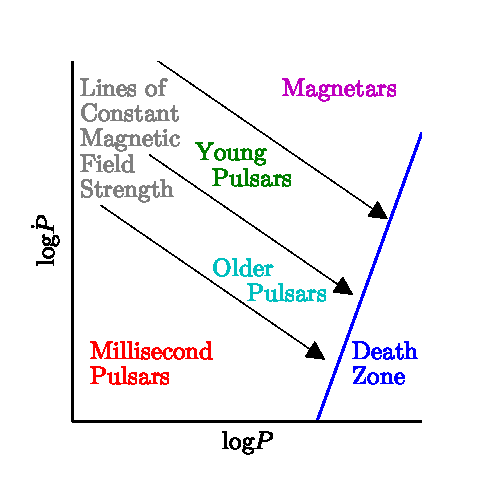
\includegraphics[width=.95\textwidth]{chapters/pulsarAnatomy/figures/ppdot.eps}
\caption[Period-period derivative schematic plot]{
\label{fig:ppdot} Period-period derivative schematic plot.}
\end{figure}

As pulsars age, their rotational period slows due to 
the loss of energy into the pulsar wind. 
Integration of Equation \ref{eq:angFreq} gives the characteristic
age of the pulsar as $t=P/2\dot{P}$
where $n=3$ or equivalently, $P\dot{P}$ is the
constant that relates $\Omega$ and $\dot{\Omega}$.
This relation is based on the assumption 
that the magnetic field
remains constant over time.

Figure~\ref{fig:ppdot} shows a schematic of various
pulsar populations.  Most pulsars start their
life in the upper left corner of the $P$--$\dot{P}$ diagram
and move diagonally downward along lines of constant
magnetic field strength.  Eventually, pulsars enter the ``death zone'' 
where they are not energetic enough to be observed.

In this thesis work, we focus on young pulsars
that are energetic enough to emit in both
radio and $\gamma$-ray wavelengths, allowing
for possible multi-wavelength studies.
Another population of pulsars that 
are energetic enough to emit in the
$\gamma$-rays are the millisecond pulsars
located in lower left corner of Figure~\ref{fig:ppdot}.

While young pulsars are rotation-powered, rotating
through the loss of rotational energy, millisecond
pulsars are accretion powered.  They are ``spun up''
by their companion star.
When the companion star of the neutron star overflows
the Roche lobe, it imparts material and angular momentum
onto the pulsar.  As a result, millisecond pulsar
periods are much faster and more 
precise compared to normal pulsar periods.










